\chapter{Application}
\label{chap:application}
\begingroup
\let\clearpage\relax

In this section, we provide an overview of the application, detailing its primary components and functionality. The app is designed to enhance user interaction through a graphical user interface (GUI), stream audio input for real-time processing, and apply our machine learning model to process the streamed audio. The application workflow is divided into two main stages before reaching the ML model: the GUI app and the streamer.

The first stage involves the GUI app, which functions as the user interface for interaction. Users input their data through this intuitive and user-friendly interface. The GUI is responsible for capturing user inputs and passing them to the subsequent stages of the application. It ensures that users can easily and effectively interact with the system, providing the necessary inputs required for further processing.

The second stage involves the streamer, which is responsible for processing real-time audio input. Its main function is to capture the user's voice. The streamer is designed to effectively handle and stream the audio data, ensuring continuous input into the system without any interruptions. This real-time streaming capability is essential for applications that require immediate audio processing and analysis.

To locate the application, please follow this link: \href{https://github.com/YoussefMagdy10/targeted-speech-enhancement-app}{targeted-speech-enhancement-app}{}. You can find the application there, along with the necessary steps to run it.

The following is an in-depth explanation of the streamer in our application, along with its key features.

\section{App Features}

In the process of developing the application, we made several key design decisions to ensure efficiency, ease of use, and robust functionality. This subsection outlines the libraries and tools chosen for the graphical user interface (GUI) and database management, and presents the technical details and components of our user interface.

\subsection{Graphical User Interface: Tkinter and CustomTkinter}

The application's graphical user interface (GUI) has been meticulously crafted using the powerful \texttt{Tkinter} library, a standard Python interface to the Tk GUI toolkit. \texttt{Tkinter} is widely recognized for its simplicity and seamless integration with Python applications, offering an object-oriented interface that simplifies the development of responsive GUI applications.

In addition to \texttt{Tkinter}, the application leverages the enhanced capabilities of \texttt{CustomTkinter} to further elevate its visual appeal and functionality. \texttt{CustomTkinter} extends the features of \texttt{Tkinter} by providing advanced customization and theming options, including support for color modes, stylish switches, and dynamic menus. Through the seamless integration of \texttt{Tkinter} and \texttt{CustomTkinter}, the application not only delivers robust performance but also boasts a modern, user-friendly interface that enhances the overall user experience.

\subsection{Database Management: SQLite}

The application utilizes SQLite, a lightweight and self-contained SQL database engine, for database management. SQLite is integrated into Python through the \texttt{sqlite3} module, which offers a straightforward interface for database operations. We opted for SQLite due to its reliability, serverless nature, and zero-configuration database solution, making it ideal for our application.

SQLite's simplicity and ease of organization are its primary advantages. It stores the entire database in a single file on the disk, ensuring high portability and easy management. Given that our stored data isn't highly complex, SQLite was the perfect choice for us.

In Python, the \texttt{sqlite3} module enables efficient execution of SQL queries, management of database connections, and handling of transactions. This makes SQLite an optimal choice for applications that require a robust database solution without the overhead of a full-fledged database server.

By leveraging \texttt{Tkinter}, \texttt{CustomTkinter}, and SQLite, the application attains a harmonious blend of functionality, performance, and user experience.

\subsection{Technical Details}

The app is designed to enhance speech using the user's reference audio. Upon first use, the client must provide their name and upload a clear voice audio from their local device.

Afterward, the client needs to select the input device for real-time voice enhancement.

Additionally, the client can adjust the percentage of noise to be removed using the dry/wet slider.

Our app supports multiple users, each mapped to one reference audio. If a user needs to replace their reference audio, they can upload a new audio file, which will replace the old one.

Once these settings have been configured, the user will be able to activate the 'Cancel Noise' switch to start noise cancellation. Switching on disables other components, as the user is not allowed to modify their values while the app is running.

If the user deactivate the 'Cancel Noise' switch, the components are enabled again and noise cancellation is halted until the user edits their necessary data and clicks activate the switch again to resume.

Finally, the app is available in both light and dark modes to suit user preferences.

\begin{figure}[h]
	\centering
	\begin{minipage}{0.45\textwidth}
		\centering
		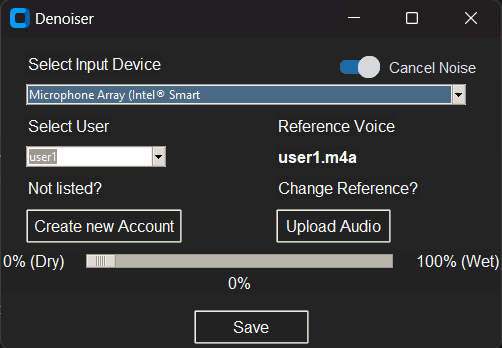
\includegraphics[width=\textwidth]{images/application/app_dark_mode.png}
		\label{fig:dark_mode}
	\end{minipage}\hfill
	\begin{minipage}{0.45\textwidth}
		\centering
		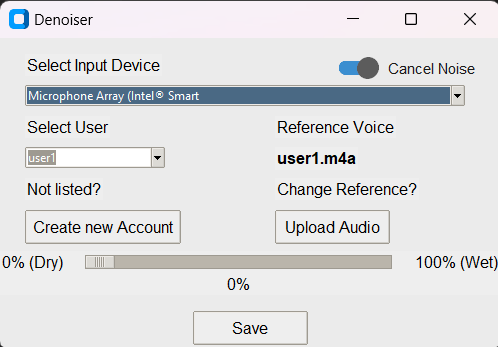
\includegraphics[width=\textwidth]{images/application/app_light_mode.png}
		\label{fig:light_mode}
	\end{minipage}
	\caption{Figure showing the appearance of our GUI in both: dark \& light mode}
	\label{fig:app_modes}
\end{figure}

Here is a recap of the features or components provided by our GUI:
\begin{itemize}
	\item \textbf{Select Input Device}: Dropdown menu that displays current audio inputs from the device.
	\item \textbf{Select User}: A dropdown menu that displays current saved usernames on the device. Once a user is selected, their reference voice's name appears next to the menu in bold.
	\item \textbf{Reference Voice}: Label that displays the user's reference audio once a user is chosen from the 'Select User' dropdown.
	\item \textbf{Create New Account}: Button that leads to another window, allowing the user to provide their name and upload their reference audio for the first time. Once this data is submitted, the user's name and reference audio remain saved in the app.
	\item \textbf{Upload Audio}: Button that enables a user to change their stored reference audio by uploading a new one.
	\item \textbf{Dry/Wet Slider}: Controls the amount of noise to keep or remove from the provided audio.
	\item \textbf{Cancel Noise}: Switch button that can be toggled on and off, initial state is 'off' while turning it on passes the given values to the model to start working.
\end{itemize}

\section{Streaming}

\begin{figure}[!t]
    \centering
    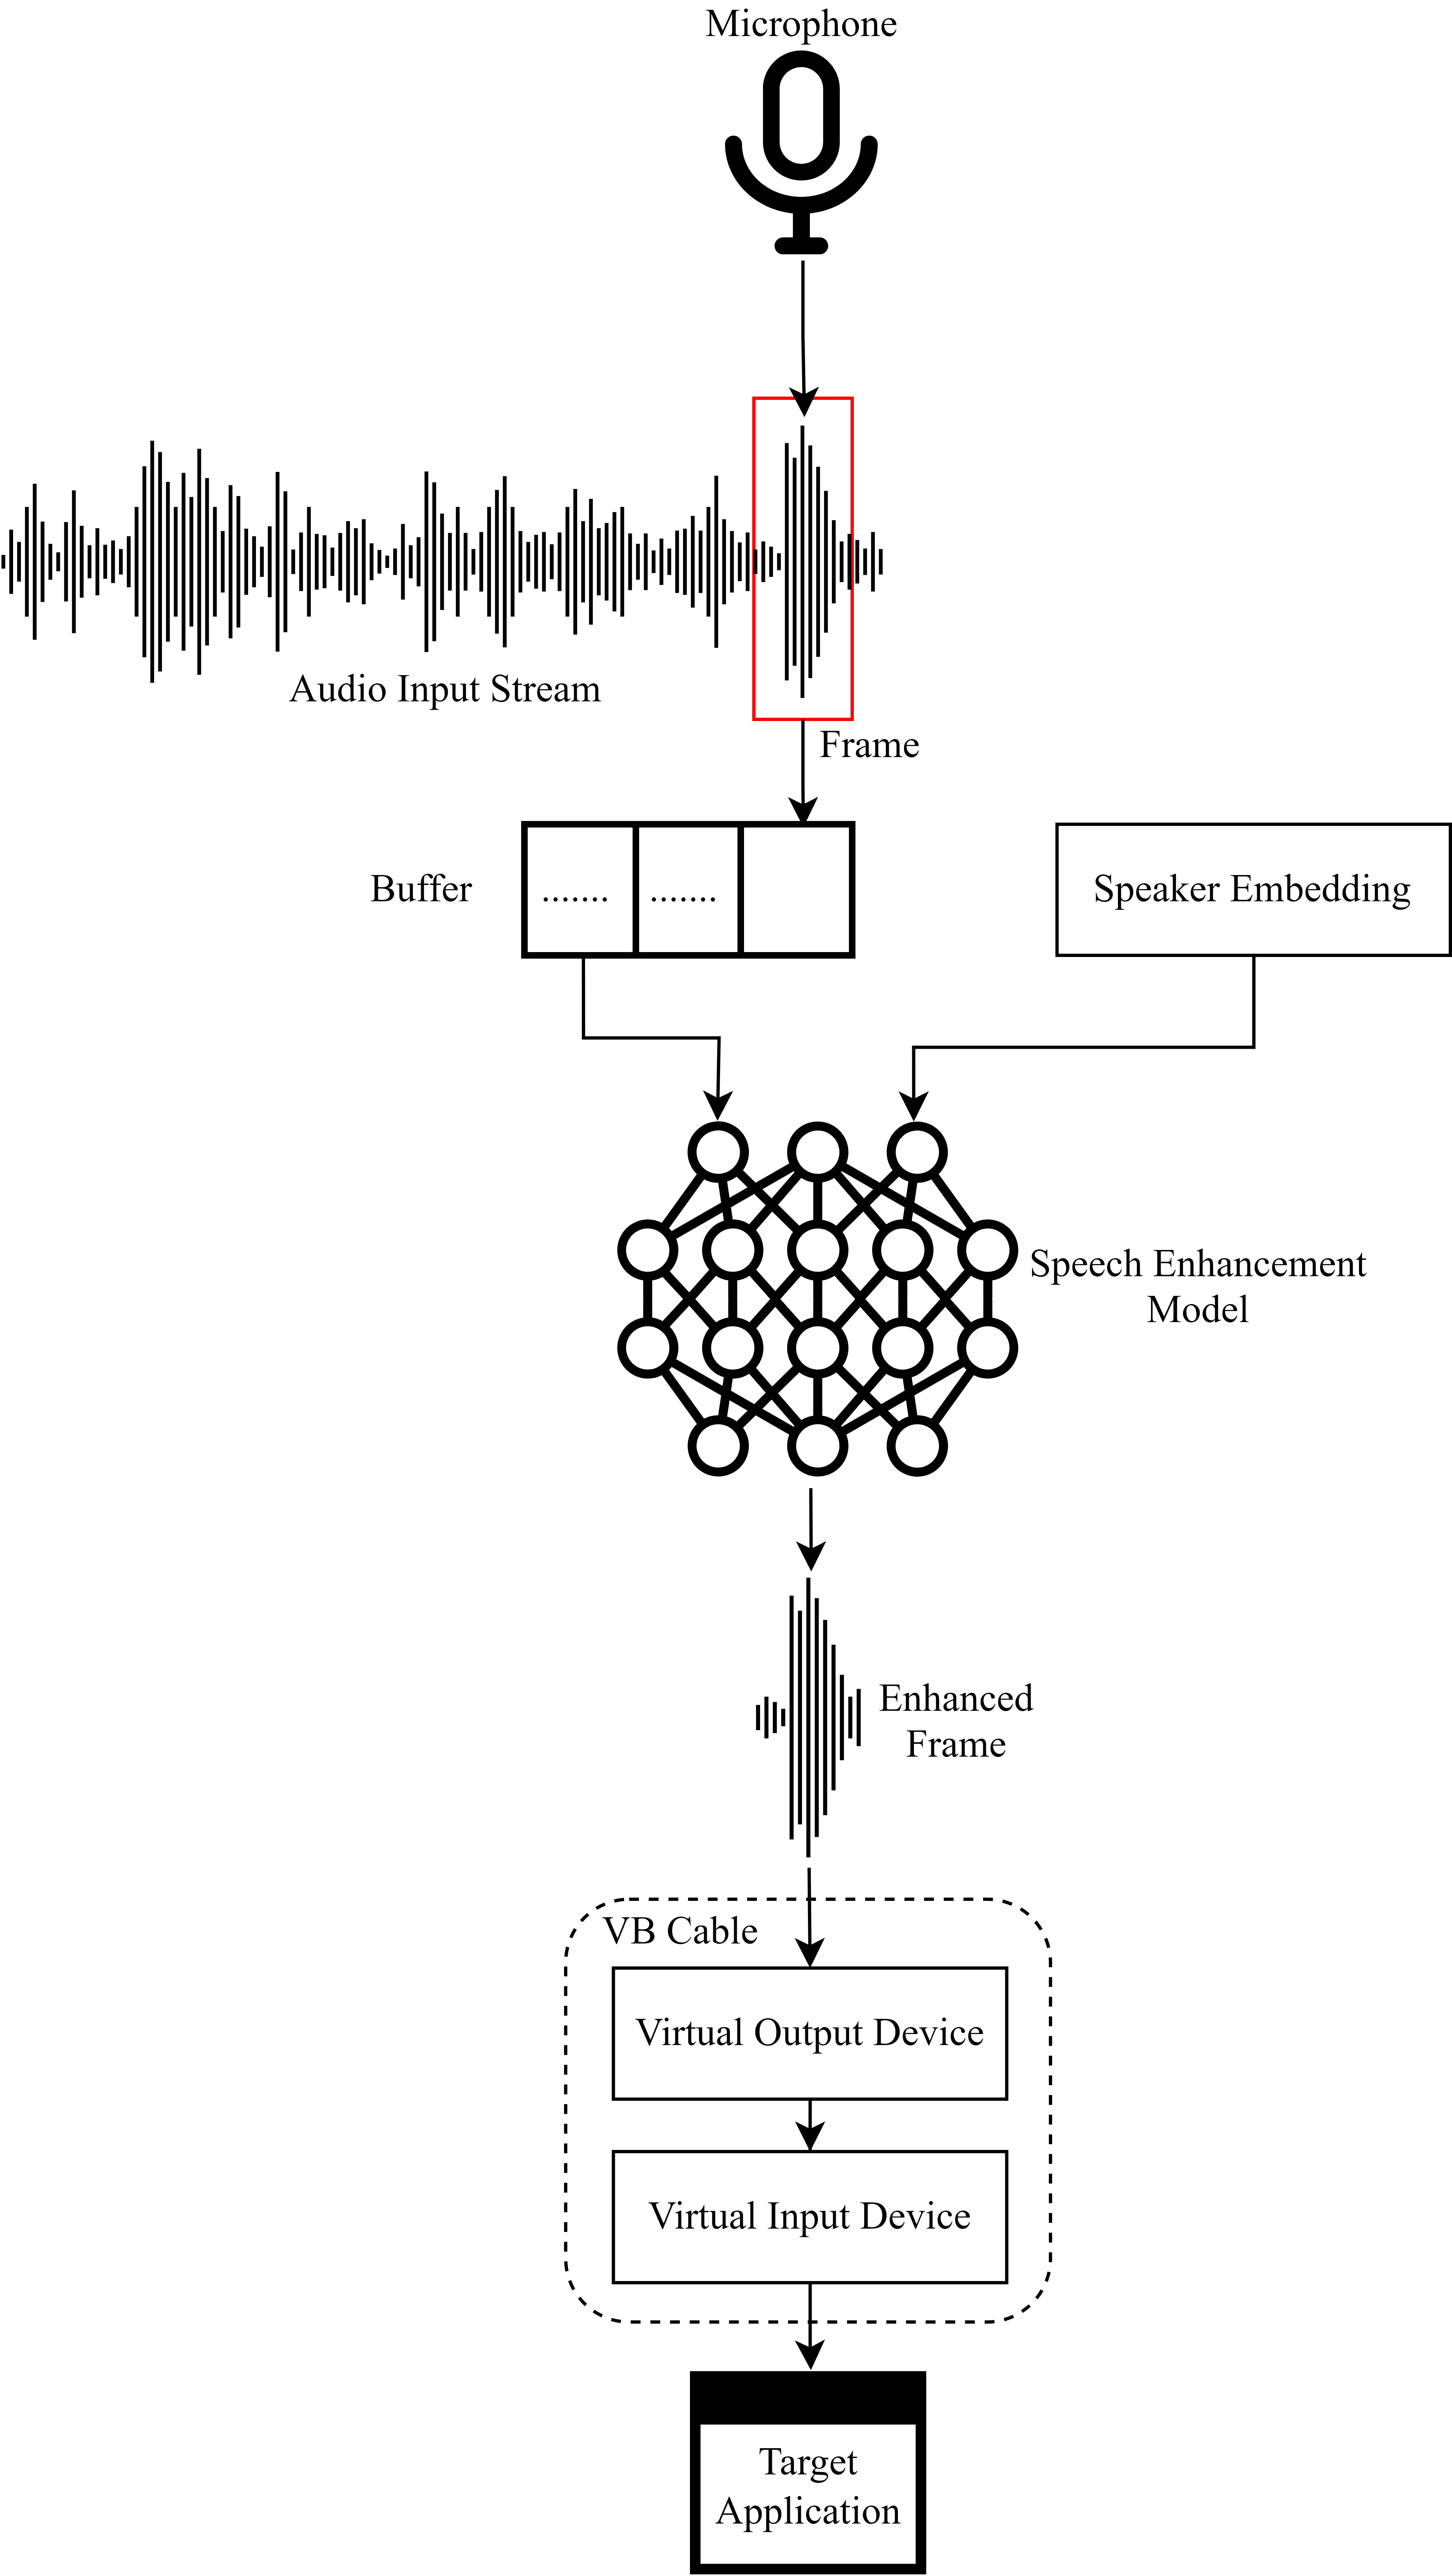
\includegraphics[width=0.8\textwidth]{images/application/streaming_pipeline.png}
    \caption{Streaming pipeline}
    \label{fig:streaming-pipeline}
\end{figure}

The streaming module is responsible for capturing real-time audio input from the user and feeding it into the machine learning model for processing. The streaming module is designed to efficiently manage and stream the audio data, ensuring that it is continuously fed into the system without interruptions. This section provides an overview of the streaming module, detailing its primary components and functionality.

The steaming pipeline starts from the user's microphone, which captures the audio input. The streaming module collects small chunks of audio data, called frames, from the microphone. Typically, the frame size is set to 60 milliseconds, however this value can be adjusted according to the application requirements. There is a trade-off between the frame size, the latency and the performance of the system. A smaller frame size will result in lower latency. Also, longer frames will result in better overall audio quality processed by the model since the model will have more context to work with but will increase the latency.

The gathered audio frames are then continuously pushed into a buffer. The buffer is a queue-like data structure that stores the audio frames in a first-in-first-out (FIFO) order. The buffer ensures that the audio frames are processed in the order they were received. Concurrent with the buffer, the streaming module continuously feeds the audio frames into the machine learning model for processing. The enhanced audio frames are then passed to the virtual output device. The virtual output device is responsible for rerouting the processed audio frames to the virtual microphone, which is then used by the user's applications as the input device. Figure \ref{fig:streaming-pipeline} shows the streaming pipeline.

In order to increase the quality of the enhanced audio, we added the option to process multiple audio frames at the same time. This increases the context the model has to work with, which results in better audio quality. As mentioned earlier, this comes at the cost of increased latency because the output device waits until $n$ full frames are gathered, making the latency as follows:
$$ \text{latency} = n \times \text{frame length} + n \times \text{processing time per frame} $$
To mitigate this, instead of keeping the streaming module idle while waiting for the model to process the audio frames, we start by processing the first frame and then save this frame for future processing. The $n-1$ saved past frames are then concatenated to the new frame to be processed by the model. This way, the streaming module can continue to collect and process audio frames without waiting for the full $n$ frames to arrive making the overall latency:
$$ \text{latency} = \text{frame length} + n \times \text{processing time} $$
This allows the streaming module to keep up with the real-time audio input and reduce the overall latency of the system. However, this approach may introduce a delay due to the added processing time of the model. This added delay is way less than the latency introduced by waiting for the full $n$ frames to arrive since the processing time is typically less than the frame length to achieve real-time constraints. We also added the option to adjust the number of working threads to process the audio frames. This far reduces the processing time of the model, which results in lower latency. If the user set the number of threads to $n$, the model will process $n$ frames at the same time, which will result in a latency of almost:
$$ \text{latency} = \text{frame length} + \text{processing time} $$
This will result in the lowest latency possible, almost the same as processing 1 frame at a time. However, it will require more processing power.

In our experiments, we set number of frames $n$ to $2$ and number of threads to $2$. This configuration resulted in a low RTF of $0.21$, which is excellent for real-time applications with low CPU utilization of $4\%$. This experiment was conducted on a laptop with CPU AMD Ryzen 9 5900HX. We can further reduce the latency and RTF by using GPU acceleration.
\endgroup
